\documentclass[conference]{IEEEtran}

\usepackage{cite}
\usepackage{amsmath,amssymb,amsfonts}
\usepackage{graphicx}
\usepackage{xcolor}
\usepackage{url}
\usepackage{booktabs}
\usepackage{makecell}
\usepackage{algorithm,algorithmic}
\usepackage{amsthm}
\usepackage{balance}

\newtheorem{proposition}{Proposition}
\newcommand{\proc}[1]{\textnormal{\textsc{#1}}}

\graphicspath{{figures/}}

\begin{document}

\title{Attack-Aware Forensic Receipts for Accountable LLM Decoding Services}

\author{
\IEEEauthorblockN{George Chidera Akor\IEEEauthorrefmark{1}, Love Allen Chijioke Ahakonye\IEEEauthorrefmark{2}, Jae Min Lee\IEEEauthorrefmark{1}, Dong-Seong Kim\IEEEauthorrefmark{1}}
\IEEEauthorblockA{\IEEEauthorrefmark{1}IT Convergence Engineering and NSLab Co. Ltd., Kumoh National Institute of Technology, Gumi, South Korea}
\IEEEauthorblockA{\IEEEauthorrefmark{2}ICT Convergence Research Center, Kumoh National Institute of Technology, Gumi, South Korea}
\IEEEauthorblockA{Corresponding author: dskim@kumoh.ac.kr}
}

\maketitle

\begin{abstract}
Operational audits of LLM services still provide limited direct evidence that decoding-time policy controls were enforced as declared. An operator or intermediary can modify top-$k$/top-$p$/temperature settings, replay randomness, reorder transcript fragments, or rewrite shortlist artifacts without leaving machine-verifiable evidence. We present an attack-aware forensic architecture that combines policy commitments, per-step receipts, tamper-evident chaining, and deterministic re-execution to verify transcript consistency with a declared decoding policy. Our prototype achieves sub-millisecond per-step latency (0.021--0.067~ms/step) and compact evidence artifacts (8--307~KB). Re-execution guarantees detection of policy mismatch, randomness replay, and transcript integrity attacks; candidate-list manipulation detection additionally requires ground-truth shortlists. A baseline comparison shows re-execution is necessary for reliable semantic attack detection (5/5 vs.\ 2/5 for the strongest alternative). We validate across 15 configurations with 0.0\% false positives (0/10{,}000) and confirm 100\% detection on real GPT-2 logit distributions across 100 diverse prompts when ground-truth shortlists are available.
\end{abstract}

\begin{IEEEkeywords}
forensic audit, stochastic decoding, tamper-evident receipts, attack detection, verifiable AI services
\end{IEEEkeywords}

\section{Introduction}
LLM services are now used in safety filtering, moderation, compliance review, and downstream decision support \cite{Inan2023LlamaGuard,Cho2024Moderators,Gu2024CoPilotedAuditing}. Regulatory frameworks such as the EU AI Act \cite{EUAIACT2024} increasingly require that high-risk AI systems maintain auditable records of their decision processes. In these deployments, accountability disputes span multiple layers, including model provenance and runtime decoding behavior. Temperature scaling, top-$k$, and nucleus sampling directly affect user-visible outputs, but these controls are still commonly treated as implementation details rather than auditable evidence \cite{holtzman2020curiouscaseneuraltext,ZKML2024}.

This creates a security gap: a malicious insider can steer outcomes by changing sampling parameters, a relay can tamper with candidate lists, and a compromised service can replay randomness \cite{Wei2024SpecSideChannel}. Prior work on blockchain-enhanced data falsification detection~\cite{Ahakonye2025DataFalsification} and explainable intrusion detection~\cite{Ahakonye2024MLExplainIDS} has addressed analogous tamper-detection and attribution problems in IoT and IIoT networks; we extend these concerns to the LLM decoding layer. Recent systems for verifiable ML have advanced forward-pass assurance \cite{Delphi2020,zkLLM2024,ZKTorch2025}, but even with authentic logits, investigators need independent evidence that the emitted transcript follows the declared policy. We therefore design a forensic audit pipeline that binds policy context, randomness context, candidate digest, selected token, and chain state at each decoding step, enabling verifiers to evaluate transcript consistency and return reason-coded outcomes. We scope guarantees to policy execution over a provided shortlist and target asynchronous verification modes \cite{Gu2024CoPilotedAuditing,Akor2025ProvAuditChain}.

\textbf{Contributions.}
(1)~A decoding-specific adversarial taxonomy with security requirements derived from incident-response needs.
(2)~A tamper-evident receipt model binding policy, randomness, candidates, and tokens into chain-of-custody artifacts.
(3)~Formal detection propositions mapping four attack classes to verifier checks.
(4)~Validation on a SHA-256 prototype across 15 configurations (0.0\% FP, sub-ms latency, 100\% detection on GPT-2 logits) with a three-baseline comparison showing re-execution is necessary for semantic attack detection.

\section{Threat Model and Security Requirements}
\subsection{System roles and trust boundaries}
We consider five roles: client, model-serving provider, receipt generator, verifier, and evidence store. The provider and receipt generator may share one administrative domain, while verifiers may be internal auditors, external assessors, or compliance services. We assume standard cryptographic hardness for commitments and proofs, but we do not assume provider-side runtime logs are inherently trustworthy.

This work targets decoding-execution accountability. It does not substitute for assurances about model training provenance, model weights, or full forward-pass correctness.

\subsection{Adversaries}
We model four attacker classes:
\begin{itemize}
\item \textbf{Compromised provider component} that modifies decoding policy parameters at runtime.
\item \textbf{Malicious relay/proxy} that tampers with candidate lists or output ordering in transit.
\item \textbf{Insider attacker} with privileged log access who attempts post-hoc evidence rewriting.
\item \textbf{Faulty automation} that unintentionally reuses randomness context or truncates transcripts.
\end{itemize}

\subsection{Assets and guarantees}
The primary assets are policy integrity, randomness integrity, candidate-list integrity, transcript continuity, and evidence chain-of-custody. Within the decoding layer, the system provides three guarantees: (i) consistency between declared policy and sampled tokens over the provided shortlist; (ii) tamper evidence for transcript edits; and (iii) failure localization signals for incident triage.

\section{Forensic Audit Architecture}
\subsection{Module overview}
The architecture contains five modules: policy registrar, receipt generator, verifier, evidence store, and incident auditor (Fig.~\ref{fig:arch}). The modules integrate with existing provenance and logging pipelines rather than replace them.

\begin{figure}[t]
\centering
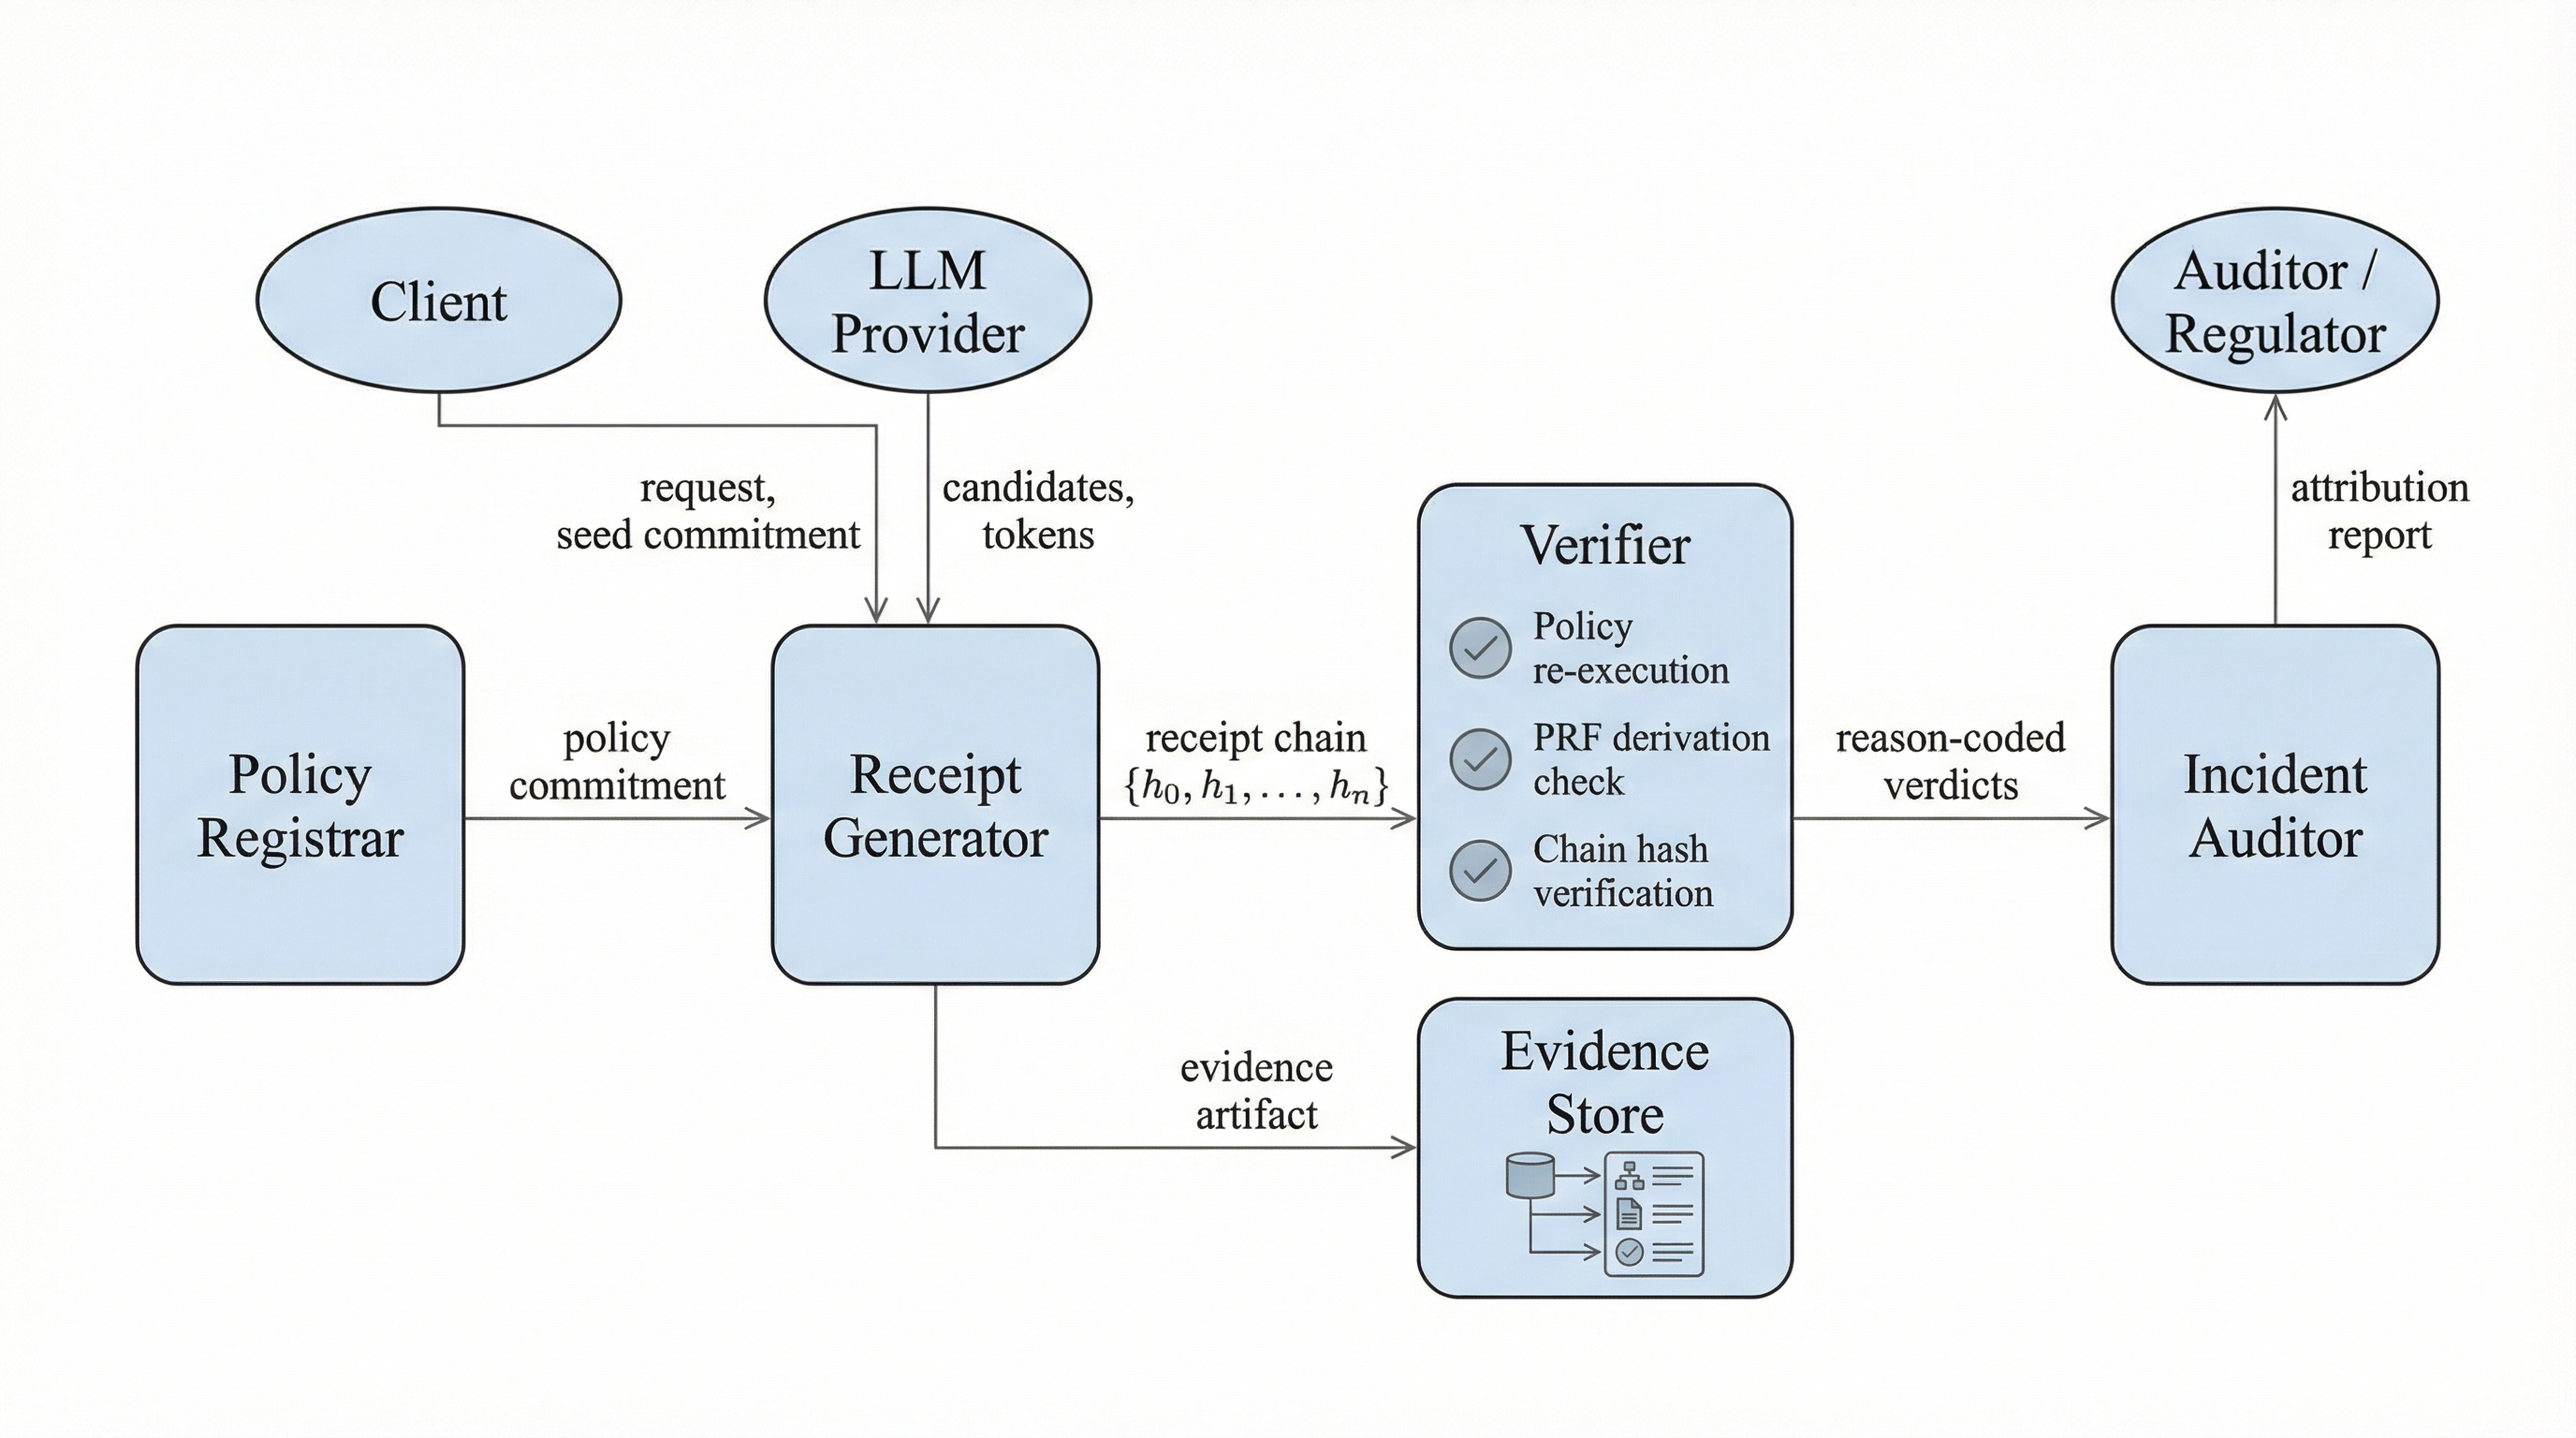
\includegraphics[width=\columnwidth]{icufn_architecture.png}
\caption{Forensic audit architecture. The receipt generator binds policy, randomness, and candidate data into a hash-chained receipt at each decoding step. The verifier re-executes decoding under committed parameters and emits reason-coded verdicts for the incident auditor.}\label{fig:arch}
\end{figure}

\begin{itemize}
\item \textbf{Policy registrar:} records versioned decoding-policy commitments and authorized update windows.
\item \textbf{Receipt generator:} emits per-step forensic receipts bound to request context.
\item \textbf{Verifier:} checks receipt-chain validity and policy-consistent decoding transitions for committed shortlist artifacts.
\item \textbf{Evidence store:} preserves receipts and proofs as immutable incident artifacts.
\item \textbf{Incident auditor:} converts verifier outcomes into attribution reports and remediation actions.
\end{itemize}

\subsection{Receipt structure and chain update}
At decoding step $t$, the system records a tuple containing request identifier, policy commitment, randomness binding, candidate digest, selected token, step index, and previous-chain hash. The chain state is updated as:
\begin{equation}\label{eq:chain}
h_t = H\!\bigl(\texttt{dom} \| h_{t-1} \| \texttt{rid} \| \texttt{ph} \| \texttt{sc} \| t \| \texttt{ch}_t \| y_t \| W^s_t \| R_t\bigr)
\end{equation}
where $H$ is SHA-256, \texttt{dom} is a domain separator, $h_{t-1}$ the previous chain hash, \texttt{rid} the request identifier, \texttt{ph} the policy hash, \texttt{sc} the seed commitment, $\texttt{ch}_t$ the candidate-set hash, $y_t$ the selected token, $W^s_t$ the sampling weight, and $R_t$ the random draw. Any change propagates to a chain mismatch.

\subsection{Verification procedure}
Algorithm~\ref{alg:verify} formalizes the verification logic. The verifier deterministically re-executes each decoding step under the committed policy, recomputes the chain hash, and emits reason-coded failures for triage.

\begin{algorithm}[t]
\caption{Transcript Verification}\label{alg:verify}
\begin{algorithmic}[1]
\REQUIRE Transcript $\mathcal{T} = \{(y_t, W^s_t, R_t, \texttt{ch}_t, h_t)\}_{t=0}^{N-1}$, policy $P$, seed $\sigma$, request id \texttt{rid}
\ENSURE Verdict $v$, failure set $\mathcal{F}$
\STATE $\mathcal{F} \leftarrow \emptyset$;\ $\hat{h} \leftarrow H(\texttt{dom}_0 \| \texttt{rid} \| \texttt{ph} \| \texttt{sc})$ \COMMENT{init receipt}
\FOR{$t = 0$ \TO $N-1$}
  \STATE $U_t \leftarrow \text{PRF}(\sigma, t)$ \COMMENT{re-derive randomness}
  \STATE $(\hat{y}_t, \hat{W}^s_t, \hat{R}_t) \leftarrow \proc{DecodeStep}(P, \texttt{cands}_t, U_t)$
  \IF{$\hat{y}_t \neq y_t$ \OR $\hat{W}^s_t \neq W^s_t$ \OR $\hat{R}_t \neq R_t$}
    \STATE $\mathcal{F} \leftarrow \mathcal{F} \cup \{(t, \proc{PolicyOrRandMismatch})\}$
  \ENDIF
  \STATE $\hat{h} \leftarrow H(\texttt{dom} \| \hat{h} \| \texttt{rid} \| \texttt{ph} \| \texttt{sc} \| t \| \texttt{ch}_t \| y_t \| W^s_t \| R_t)$
  \IF{$\hat{h} \neq h_t$}
    \STATE $\mathcal{F} \leftarrow \mathcal{F} \cup \{(t, \proc{ChainMismatch})\}$
  \ENDIF
\ENDFOR
\STATE $v \leftarrow (\mathcal{F} = \emptyset\ ?\ \proc{Pass} : \proc{Fail})$
\RETURN $(v, \mathcal{F})$
\end{algorithmic}
\end{algorithm}

\section{Attack Scenarios and Detection Logic}
We analyze four tampering scenarios detectable from decoding receipts. For each, we state a detection proposition and provide a proof sketch reducing to standard cryptographic assumptions (collision resistance of $H$, pseudorandomness of $\mathrm{PRF}$, determinism of \proc{DecodeStep}). All proofs assume that \proc{DecodeStep} is a deterministic function of its inputs and that $H$ is collision-resistant.

\subsection{Policy mismatch attack}
An attacker changes temperature or top-$p$ parameters after policy registration. Detection is triggered when recomputed transitions under committed policy fail to match receipt-declared transitions.

\begin{proposition}\label{prop:policy}
For any transcript produced with altered policy parameters $P'\!\neq\!P$, the decoding re-execution check detects the mismatch at every step where $\proc{DecodeStep}(P', \texttt{cands}_t, U_t) \neq \proc{DecodeStep}(P, \texttt{cands}_t, U_t)$, assuming \proc{DecodeStep} is deterministic and $H$ is collision-resistant.
\end{proposition}

\textit{Proof sketch.}
Since \proc{DecodeStep} is deterministic, $P'\!\neq\!P$ causes a re-execution mismatch at every step where the policy difference affects the cumulative distribution (Algorithm~\ref{alg:verify}, line~5). In the degenerate case where outputs coincide despite $P'\!\neq\!P$, two sub-cases arise: (a)~if the attacker writes $\texttt{ph}'=H(P')$ into the receipt, the chain-hash check catches the mismatch because $H(P')\!\neq\!H(P)$ under collision resistance; (b)~if the attacker writes the committed $\texttt{ph}=H(P)$ and all step outputs are identical to those under~$P$, the attack evades detection entirely, but harmlessly, since the emitted transcript is identical to honest execution.
\hfill$\square$

This guarantee holds for all perturbations that affect the cumulative distribution: our experiments confirm detection when $\delta_T$ is as small as 0.0015\% of~$T$. However, an adaptive adversary can identify \emph{degenerate steps} where $P' \neq P$ produces identical $(y, W^s_t, R_t)$, e.g., when one candidate has overwhelming probability. At such steps, the policy change is undetectable (100\% evasion at degenerate entropy, 40.9\% at medium entropy in our experiments). This is harmless: the adversary gains no utility because the output is identical to honest execution. Any perturbation that changes the output is detected with probability~1 (Section~\ref{sec:eval}).

\subsection{Randomness replay or bias attack}
An attacker reuses or manipulates randomness context to force predictable outcomes. Detection combines commitment checks with replay tests over nonce/request domains. Optional statistical alarms flag suspicious concentration patterns for analyst review.

\begin{proposition}\label{prop:rand}
Any modification to the per-step random draw $U_t$ is detected by the verifier at every step where the modified draw $U_t'$ causes $\proc{DecodeStep}(P, \texttt{cands}_t, U_t') \neq \proc{DecodeStep}(P, \texttt{cands}_t, U_t)$, assuming $\mathrm{PRF}$ security and collision resistance of $H$. Even when the outputs coincide despite $U_t' \neq U_t$, the chain-hash check detects the modification unless the attacker forges a collision.
\end{proposition}

\textit{Proof sketch.}
The verifier re-derives $U_t=\mathrm{PRF}(\sigma,t)$ from the committed seed and re-executes \proc{DecodeStep}. If $U_t'\!\neq\!U_t$ changes any intermediate quantity, the re-execution check detects the difference. In the degenerate case where outputs coincide, the attacker cannot find $\sigma'$ with $\mathrm{PRF}(\sigma',t)=U_t'$ for tampered steps while matching honest steps, by PRF security; committing to $\sigma$ exposes $U_t\!\neq\!U_t'$ at re-derivation, while committing to $\sigma'$ causes mismatches at untampered steps.
\hfill$\square$

The PRF-derivation check catches all bias attacks at any level, since the attacker must modify $U_t$ to introduce bias. A complementary statistical heuristic (Section~\ref{sec:bias}) provides a second detection layer when PRF commitments are unavailable.

\subsection{Candidate-list manipulation attack}
An attacker injects or removes shortlist entries before sampling. Detection occurs when candidate digests in receipts diverge from verifier-reconstructed digests or from signed shortlist snapshots.

\begin{proposition}\label{prop:cand}
Given ground-truth candidate sets, any substitution, injection, or removal of candidates is detected via candidate-hash mismatch, assuming $H$ is collision-resistant.
\end{proposition}

\textit{Proof sketch.}
The receipt records $\texttt{ch}_t = H(\texttt{cands}_t')$; the verifier computes $H(\texttt{cands}_t)$ from ground truth. Since $\texttt{cands}_t'\!\neq\!\texttt{cands}_t$, equality of hashes constitutes a collision, which occurs with probability $\leq 2^{-128}$ under SHA-256. Without ground-truth candidates this check is inoperative.
\hfill$\square$

Without ground-truth candidates, detection of logit-proximate substitutions (within 1 logit unit) drops to 0\%. With ground-truth candidates, detection is 100\%. This asymmetry is a key limitation discussed in Section~\ref{sec:limits}.

\subsection{Transcript truncation/reordering attack}
An attacker drops or reorders token segments before evidence handoff. Hash-chain continuity checks and step-index consistency checks expose gaps and out-of-order segments.

\begin{proposition}\label{prop:chain}
Any dropped or reordered step causes a chain-hash mismatch at the first affected position, with exact localization to the splice point, assuming $H$ is collision-resistant.
\end{proposition}

\textit{Proof sketch.}
A dropped step shifts all subsequent data by one position, causing the verifier to compute $h_t^*$ over a different prior hash and step index than the recorded $h_{t+1}$; equality would require a collision in $H$. Reordering similarly changes the step-index input at the first affected position. In both cases, the mismatch propagates by induction since each $h_t$ feeds into $h_{t+1}$.
\hfill$\square$

In transcript-splicing experiments (steps from two different requests), the verifier achieves 100\% detection and 100\% localization to the exact splice point.

\section{Related Work}

\textbf{Verifiable ML computation.}
Delphi~\cite{Delphi2020}, ZKML~\cite{ZKML2024}, ZKTorch~\cite{ZKTorch2025}, and zkLLM~\cite{zkLLM2024} prove forward-pass correctness but do not address whether decoding-layer policy controls were applied as declared; our architecture is complementary. Watermarking~\cite{Kirchenbauer2023Watermark} embeds statistical provenance signals; our approach instead provides deterministic, per-step evidence of policy compliance.

\textbf{Commitment schemes and auditable AI.}
Prediction commitments~\cite{Pinocchio2013} and co-piloted auditing workflows~\cite{Gu2024CoPilotedAuditing} make ML pipelines auditable at the model level~\cite{Kapoor2024OpenFMs}. Our receipts operate at finer granularity, binding policy, randomness, and candidate digests per decoding step.

\textbf{Blockchain and verifiable randomness.}
On-chain provenance registries~\cite{Akor2025ProvAuditChain}, VRFs~\cite{Micali1999VRF}, and scalable randomness beacons~\cite{Rondo2024} provide tamper-evident anchoring and honest-randomness guarantees. Our architecture can optionally anchor receipt roots on a ledger, and our per-step $U_t$ derivation follows a PRF pattern bound to the policy commitment, enabling replay detection without on-chain VRF verification.

\textbf{Log integrity and forensics.}
Hash-chain and Merkle-tree constructions~\cite{Crosby2009TamperEvident} underpin tamper-evident logging. Our design extends beyond passive integrity: deterministic re-execution detects policy and randomness manipulations that signed logs alone cannot distinguish from legitimate behavior.

\section{Experimental Evaluation}\label{sec:eval}

\subsection{Experimental setup}
We implement the receipt generator and verifier in Python with SHA-256 (Table~\ref{tab:params}). For scaling experiments, candidate logits are assigned by rank: the highest-ranked candidate receives logit $+2.0$ (in Q16.16 fixed-point) and the lowest receives $-3.0$, producing a peaked distribution that approximates the heavy-tailed output distributions observed in real language models. We additionally validate on logits extracted from GPT-2 (117M) across 100 prompts in four categories (e.g., ``\textit{The central bank raised interest rates by 25 basis points on}''), with $K\!=\!32$ and $N\!=\!32$ per prompt (3{,}200 total steps). All latency measurements are single-threaded. Production deployment would replace SHA-256 with Poseidon for SNARK compatibility~\cite{Nova2022}. The implementation and all experimental scripts are publicly available.\footnote{\url{https://github.com/Jupiter-Plantagenet/vrbdecode-icufn}}

\begin{table}[t]
\caption{Experimental parameters.}\label{tab:params}
\centering
\begin{tabular}{@{}ll@{}}
\toprule
Parameter & Value \\
\midrule
Language              & Python \\
Hash function         & SHA-256 (domain-separated) \\
Candidate-set sizes $K$  & 16, 32, 64 \\
Transcript lengths $N$   & 16, 32, 64, 128, 256 \\
Logit distribution    & Rank-weighted (see text) \\
Top-$k$               & $\lfloor K/4 \rfloor$ \\
Top-$p$ (Q16.16)      & 0.9 \\
Temperature (Q16.16)  & 1.0 \\
Latency runs per config & 100 (5 warmup runs discarded) \\
FP honest transcripts & 10{,}000 (incl.\ edge cases) \\
Bias heuristic FP trials & 1{,}000 \\
GPT-2 validation prompts & 100 (4 categories $\times$ 25) \\
GPT-2 attack types tested & 5 (all 4 classes; manip.\ $\pm$ GT) \\
Platform              & Intel Core i7, Ubuntu 24.04 (WSL~2) \\
\bottomrule
\end{tabular}
\end{table}

\subsection{Security analysis: baseline comparison}

We compare our forensic verifier against three baselines of increasing strength: (i)~a \emph{signed Merkle log} that records token hashes in a Merkle tree with a signed root; (ii)~a \emph{policy-commitment verifier} that binds policy parameters via hash and signs per-step records with HMAC, but does not re-execute decoding; and (iii)~a \emph{watermark-based detector} that embeds a Kirchenbauer et~al.~\cite{Kirchenbauer2023Watermark} style statistical signal by biasing sampling toward a hash-partitioned green list and testing for the signal via a one-proportion $z$-test.

Table~\ref{tab:baseline} summarizes the results across all five attack classes. The policy-commitment baseline and the Merkle baseline both detect only structural attacks; the watermark detector exhibits partial, unreliable detection because attacks that change selected tokens sometimes disrupt the green-list pattern but do not reliably do so.

\begin{table}[t]
\caption{Attack detection capability: forensic verifier vs.\ three baselines. ``Detected'' = ${\geq}99\%$ detection rate across all tested intensities. ``Partial'' = detected in some configurations but not reliably. ``Not det.'' = $0\%$ detection.}\label{tab:baseline}
\centering
\setlength{\tabcolsep}{3.0pt}
\begin{tabular}{@{}lcccc@{}}
\toprule
Attack class & \makecell{Forensic\\verifier} & \makecell{Policy-\\commit} & \makecell{Water-\\mark} & \makecell{Merkle\\log} \\
\midrule
Policy mismatch            & Detected & Not det. & Not det. & Not det. \\
Randomness replay          & Detected & Not det. & Not det. & Not det. \\
Candidate manip.\ (GT)     & Detected & Not det. & Partial  & Not det. \\
Transcript drop            & Detected & Detected & Partial  & Detected \\
Transcript reorder         & Detected & Detected & Partial  & Detected \\
\midrule
Total (reliable)           & 5/5      & 2/5      & 0/5      & 2/5 \\
\bottomrule
\end{tabular}
\end{table}

The key insight is that re-execution is necessary for detecting semantic attacks. The policy-commitment baseline binds parameters but cannot verify execution consistency; the watermark baseline detects wholesale text replacement but is blind to policy-parameter changes and randomness replay that preserve the green-list pattern. Both non-re-execution baselines detect only structural attacks (drops and reorders) via step-index checking.

\subsection{Adaptive adversary analysis}

We implement an adaptive adversary with full access to the verification algorithm, testing 200 trials across four entropy levels (degenerate, low, medium, high) at $K\!=\!16$, $N\!=\!32$. We distinguish \emph{policy evasion} (using $P'\!\neq\!P$ without detection) from \emph{output evasion} (changing the emitted token). Three strategies are evaluated. (a)~\emph{Degenerate-case search:} policy evasion exists (at degenerate entropy 100\% of perturbations produce identical outputs, declining to 40.9\% at medium entropy), but output evasion is 0\% at every entropy level, confirming that the re-execution guarantee is a hard wall with zero adversarial utility. (b)~\emph{Optimal evasion budget:} the adversary pre-screens steps and tampers only where outputs are unchanged; 100\% of steps admit such a perturbation, yet no output-changing perturbation evades detection. (c)~\emph{Collision-proximate attack:} candidate-hash Hamming distance under single-token substitution averages 128.0~bits (minimum 91~bits), providing no exploitable structure for hash collision.

\subsection{Operational metrics}

Table~\ref{tab:latency} reports verification latency, evidence size, throughput, and per-step cost across configurations. Fig.~\ref{fig:latency} visualizes the scaling behavior.

\begin{table}[t]
\caption{Verification latency and evidence size ($K$: candidate-set size, $N$: transcript length). Measured on an Intel Core i7 Desktop, Python~3.12, Ubuntu~24.04 (WSL~2), 95 measured runs per configuration after 5 warmup.}\label{tab:latency}
\centering
\setlength{\tabcolsep}{3.0pt}
\begin{tabular}{@{}rrrrrrr@{}}
\toprule
$K$ & $N$ & \makecell{Mean\\(ms)} & \makecell{P95\\(ms)} & \makecell{Size\\(KB)} & \makecell{Tput\\(t/s)} & \makecell{Per-step\\(ms)} \\
\midrule
16 &  16 & 0.35 & 0.40 &  8.4 & 2{,}899 & 0.022 \\
16 &  64 & 1.51 & 2.15 & 32.3 &    662 & 0.024 \\
16 & 256 & 5.65 & 8.91 &128.4 &    177 & 0.022 \\
\midrule
32 &  16 & 0.59 & 0.69 & 12.1 & 1{,}686 & 0.037 \\
32 &  64 & 2.37 & 2.95 & 47.3 &    421 & 0.037 \\
32 & 256 & 9.31 &10.13 &188.4 &    107 & 0.036 \\
\bottomrule
\end{tabular}
\end{table}

\begin{figure}[t]
\centering
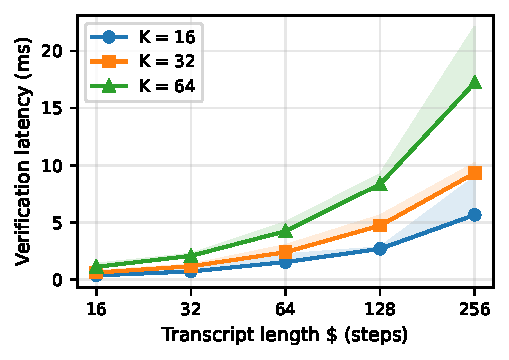
\includegraphics[width=\columnwidth]{latency_vs_n.pdf}
\caption{Verification latency vs.\ transcript length $N$ for $K \in \{16, 32, 64\}$. Shaded bands indicate P95 latency. Scaling is linear in $N$.}\label{fig:latency}
\end{figure}

\textbf{Scaling behavior.} Latency scales linearly with $N$ and sub-linearly with $K$ ($1.7\times$ per-step cost when doubling $K$ from 16 to 32), confirming $O(N)$ complexity with no hidden superlinear factors (Fig.~\ref{fig:latency}). Evidence sizes range from 8.4~KB ($K\!=\!16$, $N\!=\!16$) to 306.8~KB ($K\!=\!64$, $N\!=\!256$).

\subsection{Correctness validation}

Detection follows from Propositions~\ref{prop:policy}--\ref{prop:chain}: any deviation in $P$, $U_t$, or step ordering produces a mismatch, with security reducing to collision resistance and PRF pseudorandomness. Degenerate cases where outputs coincide despite parameter changes are harmless (identical to honest execution) as discussed in Proposition~\ref{prop:policy}. We validate across all 15 $(K,N)$ configurations, confirming 100\% detection when at least one tampered step is present.

\textbf{False-positive rate.} We measure the FP rate across 10{,}000 honest transcripts spanning all $(K, N)$ configurations and edge cases (near-boundary top-$p$, extreme temperature $T\!=\!1$, all-ties logits, minimal $K\!=\!1$). The observed rate is 0/10{,}000; a 95\% Wilson confidence interval gives $[0.0\%,\, 0.038\%]$.

\subsection{Bias heuristic characterization}\label{sec:bias}

As a complementary detection layer, we evaluate a statistical heuristic that flags transcripts where any single token ID is selected more than $\max(N/2, 8)$ times, indicating potential selection bias.

Under Zipf-like distributions modeling honest decoding, the false-positive rate is 0.0\% (0/1{,}000 honest transcripts). Fig.~\ref{fig:bias} shows the detection characteristic: the heuristic exhibits a step function at $p = 0.5$, with 0\% detection for $p < 0.5$ and 100\% for $p \geq 0.5$. Overall detection (including the PRF check) is 100\% at all bias levels, since the attacker must modify $U_t$ to inject bias. This sharp transition means the heuristic alone is effective against strong bias but does not detect subtle distributional steering.

\begin{figure}[t]
\centering
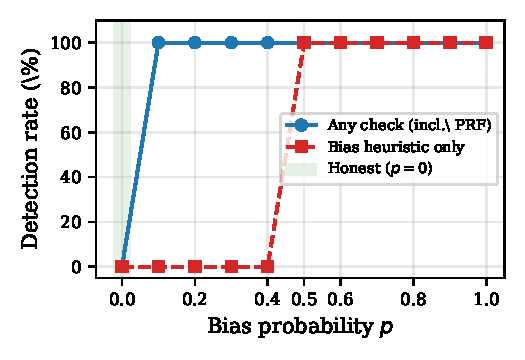
\includegraphics[width=\columnwidth]{bias_detection.pdf}
\caption{Bias detection power vs.\ bias probability $p$ ($K\!=\!16$, $N\!=\!32$). The PRF-derivation check catches all bias levels; the statistical heuristic adds a second detection layer with a step-function threshold at $p = 0.5$.}\label{fig:bias}
\end{figure}

\subsection{Validation with real LLM logits}\label{sec:gpt2}

We validate on real logit distributions extracted from GPT-2 (117M) across 100 prompts in four categories (25 per category, 3{,}200 total steps), testing all four attack types with 95\% Wilson CIs.

\textbf{Honest verification.} All 100 honest transcripts pass verification (FP rate 0.0\%, 95\% Wilson CI $[0.0\%,\, 3.7\%]$).

\textbf{Attack detection.} Table~\ref{tab:gpt2attacks} reports detection rates. All four attack types with ground-truth shortlists achieve 100\% detection ($[96.3\%,\, 100.0\%]$). Candidate manipulation without ground truth achieves 53\% ($[43.3\%,\, 62.5\%]$), confirming the trust boundary in Section~\ref{sec:limits}.

\begin{table}[t]
\caption{GPT-2 attack detection rates (100 prompts, $K\!=\!32$, $N\!=\!32$).}\label{tab:gpt2attacks}
\centering
\begin{tabular}{@{}lrrl@{}}
\toprule
Attack type & Det. & Total & Rate (95\% Wilson CI) \\
\midrule
Policy mismatch ($T/2$) & 100 & 100 & 100.0\% $[96.3,\, 100.0]$ \\
Randomness replay       & 100 & 100 & 100.0\% $[96.3,\, 100.0]$ \\
Candidate manip.\ (GT)  & 100 & 100 & 100.0\% $[96.3,\, 100.0]$ \\
Candidate manip.\ (no GT) & 53 & 100 & 53.0\% $[43.3,\, 62.5]$ \\
Transcript drop (50\%)  & 100 & 100 & 100.0\% $[96.3,\, 100.0]$ \\
\bottomrule
\end{tabular}
\end{table}

\textbf{Entropy analysis.} Real logit distributions exhibit wider per-step entropy variation than our Zipf approximation, ranging from 0.001~bits (near-deterministic code completions) to 4.95~bits (open-ended conversational), with an overall mean of 2.81. The verification pipeline handles this full entropy range without false positives.

\textbf{Latency.} Honest verification latency on real GPT-2 transcripts averages 1.19~ms per transcript (0.037~ms/step, 95\% CI $[1.17,\, 1.21]$~ms), consistent with the synthetic scaling results in Table~\ref{tab:latency}.

\section{Limitations}\label{sec:limits}
The architecture has six limitations:
(1)~candidate-list manipulation detection requires ground-truth shortlists;
(2)~at degenerate steps, harmless policy evasion is possible (identical outputs under $P'\!\neq\!P$) but output-changing evasion is 0\%;
(3)~the bias heuristic cannot detect subtle bias at $p<0.5$;
(4)~SHA-256 is not ZK-friendly; production requires Poseidon;
(5)~floating-point non-determinism across platforms could cause spurious mismatches;
(6)~evidence sizes grow linearly with $K$ and $N$.

\section{Conclusion}
We presented an attack-aware forensic architecture for accountable LLM decoding services. Deterministic re-execution guarantees detection of policy mismatch, randomness replay, and transcript integrity attacks; candidate-list manipulation additionally requires ground-truth shortlists. A three-baseline comparison confirms re-execution is necessary for semantic attack detection (5/5 vs.\ 2/5). Validation across 15 configurations yields 0.0\% false positives (0/10{,}000), sub-millisecond per-step latency, and 100\% detection on GPT-2 logits from 100 prompts with compact evidence artifacts (8--307~KB). Future work targets Poseidon-based hashing for SNARK integration, cross-platform determinism testing to characterize floating-point mismatch rates, and field evaluation in production LLM serving pipelines with real-time audit workflows.

\balance
\bibliographystyle{IEEEtran}
\bibliography{refs}

\end{document}
